\documentclass[tikz]{standalone}

\usepackage{tikz}

\begin{document}
\begin{tikzpicture}[
        every node/.style={draw, rounded corners=5pt, minimum size=1.5cm, inner sep=5pt},
        every path/.style={thick}
    ]
    \newcommand{\imagenode}[3]{ % #1 = Chapter label/dir, #2 = position, #3 Chapter title
            \node (#1) at #2
            [label=above:\raisebox{-3em}{{\parbox{4em}{\centering \tiny #3}}}]
            {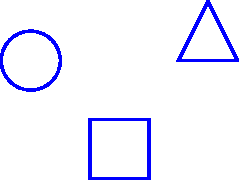
\includegraphics[width=4em]{../../../#1/logo/main.pdf}};
    }

    % First row of chapters
    \imagenode{games}{(-3, 1)}{Chapter 1: Games}
    \imagenode{rationalisation}{(-3, -3)}{Chapter 2: Rationalisation}

    % Edges showing relationships
    \draw[->] (games) to [out=-135, in=135] (rationalisation);

\end{tikzpicture}
\end{document}
